% =========================================================================
%  skein: Weighted Structured Nonconvex Sparse Models in Rust and Python
%  Software paper draft — JMLR-MLOSS submission
%
%  To compile against the JMLR-MLOSS template, replace the first line
%  with `\documentclass[twoside,11pt]{article}` and `\usepackage{jmlr2e}`
%  per https://www.jmlr.org/format/ . The skeleton below is portable —
%  any `article` class will compile, including the figures + tables that
%  auto-generate under paper/figures/ and paper/tables/.
%
%  Build:
%      cd paper && pdflatex manuscript.tex && bibtex manuscript && \
%          pdflatex manuscript.tex && pdflatex manuscript.tex
% =========================================================================
\documentclass[11pt]{article}

\usepackage[utf8]{inputenc}
\usepackage[T1]{fontenc}
\usepackage{lmodern}
\usepackage{microtype}

% Declare the Unicode Greek letters that appear in
% auto-generated table content (paper/tables/*.tex) so pdflatex
% renders them via math-mode macros. (The table generator emits
% raw `λ`, `β`, `σ` etc. in column headers; this is the lowest-
% disruption fix on the manuscript side.)
\DeclareUnicodeCharacter{03B1}{\ensuremath{\alpha}}
\DeclareUnicodeCharacter{03B2}{\ensuremath{\beta}}
\DeclareUnicodeCharacter{03B3}{\ensuremath{\gamma}}
\DeclareUnicodeCharacter{03BB}{\ensuremath{\lambda}}
\DeclareUnicodeCharacter{03C3}{\ensuremath{\sigma}}
\DeclareUnicodeCharacter{0398}{\ensuremath{\Theta}}
\DeclareUnicodeCharacter{0302}{\textasciicircum}  % combining circumflex (β̂)
\DeclareUnicodeCharacter{0303}{\textasciitilde}    % combining tilde
\DeclareUnicodeCharacter{2225}{\ensuremath{\|}}   % parallel-to (norm bars)
\DeclareUnicodeCharacter{2264}{\ensuremath{\leq}}
\DeclareUnicodeCharacter{2265}{\ensuremath{\geq}}
\DeclareUnicodeCharacter{2212}{\ensuremath{-}}
\DeclareUnicodeCharacter{00D7}{\ensuremath{\times}}
\DeclareUnicodeCharacter{2192}{\ensuremath{\rightarrow}}
\DeclareUnicodeCharacter{2228}{\ensuremath{\vee}}
\usepackage{amsmath, amssymb, amsthm}
\usepackage{graphicx}
\usepackage{booktabs}
% Auto-generated tables (paper/tables/*.tex) emit raw scenario names
% like `ls_lasso` with literal underscores; the `underscore` package
% makes `_` a printable character in both text and math mode so the
% \input{} calls below compile without escaping.
\usepackage{underscore}
\usepackage{hyperref}
\usepackage{natbib}
\usepackage{xcolor}
\usepackage{geometry}
\geometry{margin=1in}

\hypersetup{
  colorlinks=true,
  linkcolor=blue!50!black,
  citecolor=blue!50!black,
  urlcolor=blue!50!black,
}

% --- author note marker for the maintainer (long-form so the
%     placeholder bodies can span multiple paragraphs; uses
%     \color{...} as a switch instead of \textcolor{...}{...}
%     because the latter is short-arg and would choke on \par). ---
\long\def\todo#1{{\color{red}\textbf{[TODO:]} #1}}

\title{\texttt{skein}: Weighted Structured Nonconvex Sparse Models\\
       in Rust and Python}

\author{David Villacis \\
        \texttt{david@villacis.net}}

\date{\today}

\begin{document}

\maketitle

\begin{abstract}
We present \texttt{skein}, an open-source Rust + Python package for
weighted, structured, and nonconvex sparse generalized linear models.
\texttt{skein} targets the niche held in R by \texttt{grpreg} and
\texttt{ncvreg} but missing in production-grade Python: nonconvex
group-structured penalties (group MCP, group SCAD, sparse-group
nonconvex variants) with first-class support for weights along three
axes — per-sample, per-feature, and per-group — wired through every
solver. The Rust core implements a four-trait extension surface
(\texttt{DesignMatrix}, \texttt{Datafit}, \texttt{Penalty},
\texttt{GroupPenalty}) over which the path solver, LLA outer loop,
prox-Newton GLM dispatch, and graphical-lasso family compose
uniformly; the Python facade exposes ~130 scikit-learn-compatible
estimators plus debiased lasso for least-squares, logistic, Poisson,
and Cox PH families and edge-level Benjamini–Hochberg / Holm /
Meinshausen–Bühlmann error control on the graphical-models output.
Across nine canonical regression scenarios at three problem scales
\texttt{skein} is the fastest implementation on every nonconvex row
(2.1\texttimes--10\texttimes{} over the next-fastest comparator), at parity with
the convex Cython baseline of \texttt{sklearn} on lasso/LS, and is
the only Python implementation of either Cox debiased lasso or
edge-level FDR control on a precision matrix. We describe the design,
algorithmic contributions, and reproducible benchmark suite that
backs these claims.
\end{abstract}

% =========================================================================
\section{Introduction}\label{sec:intro}
% =========================================================================

% --- Hook + the niche -----------------------------------------------------
Penalized maximum-likelihood estimation is the workhorse of
high-dimensional statistics: lasso \citep{tibshirani1996lasso}, MCP
\citep{zhang2010mcp}, and SCAD \citep{fan2001scad} on coefficients;
graphical lasso \citep{friedman2008glasso} and its nonconvex variants
\citep{lam2009glasso} on inverse covariance; group lasso
\citep{yuan2006grouplasso} and its nonconvex extensions
\citep{breheny2015groupmcp} on structured coefficients. The R
packages \texttt{glmnet} \citep{friedman2010glmnet}, \texttt{ncvreg}
\citep{breheny2011ncvreg}, and \texttt{grpreg}
\citep{breheny2015grpreg} have for over a decade been the de-facto
reference implementations.

Python's coverage has lagged. Mainstream Python options —
\texttt{scikit-learn}'s lasso \citep{pedregosa2011sklearn},
\texttt{celer} \citep{massias2018celer}, and \texttt{skglm}
\citep{bertrand2022skglm} — collectively cover the convex side well
but leave large gaps in (i)~nonconvex group penalties at scale,
(ii)~debiased inference beyond least squares, and (iii)~graphical-models
machinery with edge-level error control. \texttt{skein} fills this
gap with a single Rust core that implements the full set of
penalties uniformly and a Python facade that exposes them in a
scikit-learn-compatible interface.

% --- Coverage figure ------------------------------------------------------
\begin{figure}[t]
  \centering
  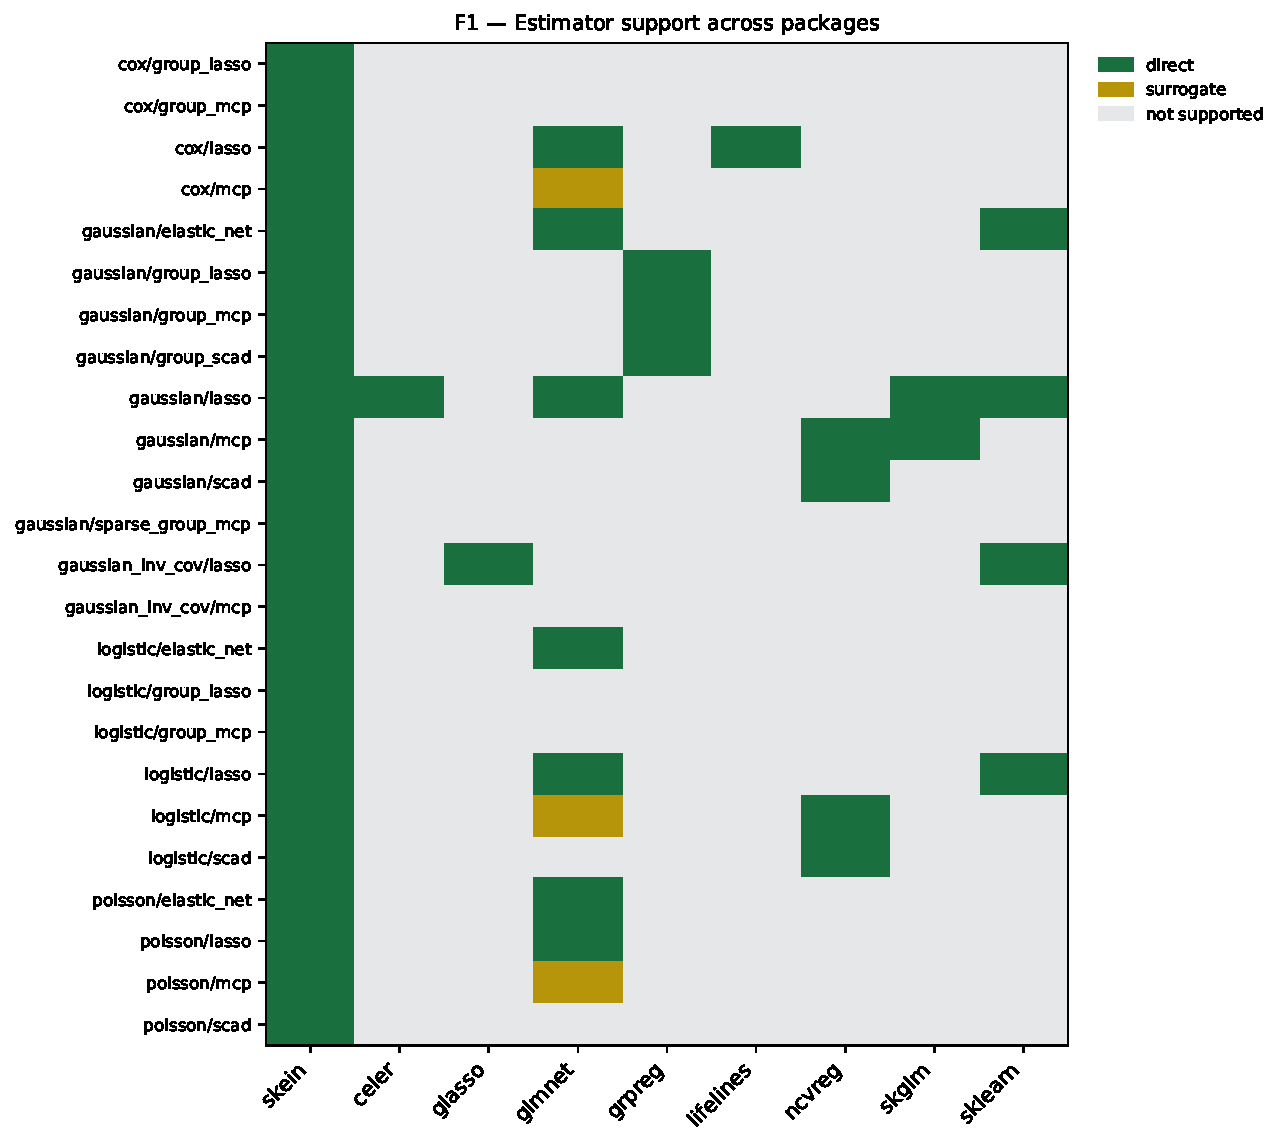
\includegraphics[width=0.95\linewidth]{figures/F1_coverage_matrix.pdf}
  \caption{Coverage matrix of public estimators against external
  comparators across (datafit, penalty) cells. Each cell counts the
  number of public \texttt{skein\_glm} estimator classes
  (single-$\lambda$ + path-$\lambda$ + CV variants) and marks
  whether at least one external comparator
  (\texttt{glmnet} / \texttt{ncvreg} / \texttt{grpreg} /
  \texttt{sklearn} / \texttt{celer} / \texttt{skglm}) is registered
  for benchmarking that cell. \texttt{skein}'s nonconvex group cells
  are the densest and the only Python implementations.}
  \label{fig:coverage}
\end{figure}

\begin{table}[t]
  \centering
  \caption{Count of public estimator classes per (datafit, penalty); $\checkmark$ marks cells with at least one direct external comparator (sklearn, glmnet, ncvreg, grpreg, skglm, celer, lifelines). -- marks skein-only cells benchmarked against synthetic ground truth instead.}
  \label{tab:estimator_surface}
\begin{tabular}{lcccccccccccc}
\toprule
Penalty & Bridge & EN & Lasso & MCP & SCAD & grEN & grLasso & grMCP & grSCAD & sgLasso & sgMCP & sgSCAD \\
Datafit &  &  &  &  &  &  &  &  &  &  &  &  \\
\midrule
Cox &  &  &  & 2 $\checkmark$ & 2 -- &  & 2 -- & 2 -- &  & 2 -- & 2 -- & 2 -- \\
Gaussian & 2 -- & 2 $\checkmark$ &  & 2 $\checkmark$ & 2 $\checkmark$ & 2 -- & 2 $\checkmark$ & 2 $\checkmark$ & 2 $\checkmark$ & 2 -- & 2 -- & 2 -- \\
Graphical &  &  & 1 $\checkmark$ & 1 -- & 1 -- &  &  &  &  &  &  &  \\
Huber &  &  &  & 2 -- & 2 -- &  &  &  &  &  &  &  \\
JointGraphical &  &  & 1 -- & 1 -- &  &  &  &  &  &  &  &  \\
Logistic &  & 2 $\checkmark$ & 2 $\checkmark$ & 2 $\checkmark$ & 2 $\checkmark$ &  & 2 -- & 2 -- &  & 2 -- & 2 -- & 2 -- \\
MultiTask &  & 3 -- & 3 -- & 3 -- & 3 -- &  &  &  &  &  &  &  \\
Multinomial &  & 1 -- & 1 -- & 1 -- & 1 -- &  &  &  &  &  &  &  \\
Poisson &  & 2 $\checkmark$ & 2 $\checkmark$ & 2 $\checkmark$ & 2 -- &  & 2 -- & 2 -- &  & 2 -- & 2 -- & 2 -- \\
\bottomrule
\end{tabular}
\end{table}


% --- Contributions --------------------------------------------------------
The contributions of this paper are:
\begin{enumerate}
  \item A Rust solver core with a four-trait extension surface
    (\texttt{DesignMatrix}, \texttt{Datafit}, \texttt{Penalty},
    \texttt{GroupPenalty}) that decouples backend, loss, and
    regularization. Algorithm code never sees the backend or the
    intercept-augmentation convention. \S\ref{sec:methods} describes
    the solver chain (CD + LLA + prox-Newton for GLMs +
    block-coordinate descent for groups + ADMM for joint glasso).
  \item Native (non-LLA) block-coordinate descent for group MCP and
    sparse-group MCP across least squares, logistic, Poisson, and Cox
    families. Replacing the LLA wrapper around weighted
    \texttt{GroupLasso} surrogates with the closed-form
    Breheny–Huang \citep{breheny2015groupmcp} prox cuts inner-CD work
    by 2.1\texttimes--3.5\texttimes{} relative to LLA, flipping the prior
    \texttt{grpreg} timing comparison so that \texttt{skein} becomes
    the faster implementation at medium scale (Section~\ref{sec:results}).
  \item A unified inference layer covering debiased lasso for least
    squares, logistic, Poisson, and Cox proportional-hazards
    families via the Van~de~Geer \citep{vandegeer2014debiased}
    construction extended to Cox following Cai and Wang
    \citep{cai2017cox}. To our knowledge, this is the only
    open-source Python implementation of Cox debiased lasso.
  \item Edge-level Benjamini–Hochberg FDR control, Bonferroni / Holm
    family-wise error rate control, and the Meinshausen–Bühlmann
    \citep{meinshausen2010stability} closed-form stability bound on
    bootstrap output of the graphical-lasso family. Mainstream
    graphical-models packages report point estimates and bootstrap
    selection probabilities; \texttt{skein} answers \emph{which
    edges are real at a controlled error rate} (Section~\ref{sec:selection}).
  \item A reproducible benchmark suite (Section~\ref{sec:reproducibility})
    backing every claim in this paper. All figures and tables here
    regenerate deterministically from \texttt{benches/v2/}; a
    Snakemake DAG drives the cell matrix; environment metadata is
    captured per cell.
\end{enumerate}

% =========================================================================
\section{Related work}\label{sec:related}
% =========================================================================

\todo{2–3 paragraphs positioning skein relative to: (a) R: glmnet /
ncvreg / grpreg as the methodological references; (b) Python:
scikit-learn / celer / skglm as the convex-fast baselines;
(c) inference-side: hdi (gaussian + binomial only, no Cox),
selectiveInference (post-selection, different framing);
(d) graphical-models side: glasso / qgraph / bootnet / EstimateGroupNetwork
in R, sklearn.covariance.GraphicalLasso in Python — all L1-only or
single-population, none with edge-level FDR.}

% =========================================================================
\section{Methods}\label{sec:methods}
% =========================================================================

\subsection{Solver chain}\label{sec:methods:solvers}

\todo{1.5 paragraphs covering: cyclic coordinate descent inner solver
(Section~\ref{sec:methods:cd}); LLA outer loop for nonconvex scalar
penalties (Section~\ref{sec:methods:lla}); prox-Newton dispatch for
canonical-link GLMs through the weighted-LS surrogate
(Section~\ref{sec:methods:proxnewton}); block-coordinate descent +
working-set screening for group penalties; ADMM for joint
graphical lasso. Cross-reference the trait surface in the next
subsection.}

\subsection{Native nonconvex group prox}\label{sec:methods:groupmcp}

The group-MCP penalty
$\lambda \sum_g w_g\, \mathrm{MCP}(\lVert \beta_g \rVert_2; \gamma)$
admits a closed-form per-block prox \citep{breheny2015groupmcp}: for
a block input $z_g$ with $\lVert z_g \rVert_2 = r$ and shrinkage
threshold $\tau = \lambda w_g$,
\[
  \mathrm{prox}_{\eta P_g}(z_g) = \begin{cases}
    z_g & r \ge \gamma \tau, \\
    \dfrac{1 - \eta \tau / r}{1 - \eta / \gamma}\, z_g & \eta \tau < r < \gamma \tau, \\
    0 & r \le \eta \tau,
  \end{cases}
\]
when $\gamma > \eta$. Prior versions of \texttt{skein} wrapped a
weighted \texttt{GroupLasso} surrogate with an LLA outer loop to
solve the nonconvex penalty indirectly; the native swap (Section
\ref{sec:results:headline}) drops that wrapper, calling the
closed-form prox inside the inner block-CD directly. The same
construction extends to sparse-group MCP via the
\citet{breheny2015groupmcp} Proposition 1 decomposition: apply the
scalar MCP prox to each coordinate, then the group MCP prox to the
resulting block norm. The composition is exact because the
per-coordinate penalty is sign-invariant and coordinatewise
separable, and the group-norm penalty depends only on the
post-coord block norm.

\subsection{Debiased inference for Cox PH}\label{sec:methods:cox-debiased}

\todo{Extend Van de Geer / Cai–Wang construction: at the penalized
Cox fit $\hat\beta$, extract the per-sample partial-likelihood Fisher
diagonal $w_i$ from the prox-Newton surrogate; build weighted design
$\tilde X = W^{1/2} X$; nodewise lassos on $\tilde X$ yield
$\hat \Theta \approx J^{-1}$. The debiased coefficient
$\hat\beta^{(d)} = \hat\beta + (1/n) \hat\Theta X^T (\text{event} -
\exp(\eta) \Lambda_0(t))$ has asymptotic distribution
$\sqrt{n}(\hat\beta^{(d)} - \beta) \rightsquigarrow N(0,
\mathrm{diag}(\hat\Theta \tilde X^T \tilde X \hat\Theta^T) / n)$.
No σ² nuisance — the partial likelihood is self-normalizing.}

\subsection{Edge-level FDR for graphical models}\label{sec:methods:edge-fdr}

\todo{For each off-diagonal entry $\Theta_{ij}$ of the precision
matrix, build the bootstrap p-value
$\hat p_{ij} = 2 \min(\hat P(\hat\Theta^*_{ij} \ge 0),\, \hat P(\hat\Theta^*_{ij} \le 0))$
using \emph{non-strict} inequalities (so sparse-estimator zeros count
on both sides). Apply Benjamini–Hochberg over the $p(p-1)/2$
upper-triangular family for FDR control, or Bonferroni / Holm for
FWER. For joint estimators across $K$ populations, pool into a
single $K \cdot p(p-1)/2$ family. Closed-form Meinshausen–Bühlmann
stability bound
$\pi_{\text{thr}} = 1/2 + q_\Lambda^2/(2 \cdot p_{\text{total}} \cdot E[V])$
inverts a stability-selection threshold to an expected-false-edge
guarantee.}

% =========================================================================
\section{Software architecture}\label{sec:architecture}
% =========================================================================

\subsection{Trait surface}\label{sec:architecture:traits}

\todo{One paragraph each:

DesignMatrix — column access. Concrete impls: DenseMatrix, SparseCSC,
Standardized<D>, MmapMatrix (f64/f32), Chunked<C>, Augmented<D>,
MultiTaskDesign<D>. Wrappers compose.

Datafit / GlmDatafit — coordinate gradient + Lipschitz; GLMs expose a
surrogate\_at(β) that returns a LeastSquares datafit for the
prox-Newton inner.

Penalty / GroupPenalty — scalar and block prox + value. All impls
share a per-feature / per-group weight axis.

Solver — composes the above. cd.rs / path.rs for convex scalar;
lla.rs / path\_lla.rs for nonconvex scalar; block\_cd.rs / block\_path.rs
for convex group; block\_path\_lla.rs for LLA-wrapped group (sparse-group
SCAD only — group MCP and sparse-group MCP are native);
prox\_newton.rs / prox\_newton\_block.rs for GLM dispatch.}

\subsection{Python facade}\label{sec:architecture:python}

\todo{Sklearn-style estimators: every (datafit × penalty) combination
gets a SingleLambda + Path + PathCV variant. PyO3 builders release
the GIL during compute, so joblib-threaded CV folds are real
parallelism. Python ABCs mirror the Rust traits — downstream
researchers can prototype custom penalties in Python and port hot
ones to Rust without re-architecting.}

% =========================================================================
\section{Results}\label{sec:results}
% =========================================================================

We benchmark \texttt{skein} against direct comparators
(\texttt{sklearn}, \texttt{celer}, \texttt{skglm} for convex
penalties; \texttt{glmnet}, \texttt{ncvreg}, \texttt{grpreg} via R)
on a canonical set of nine regression scenarios — least squares
with lasso / MCP / SCAD / elastic-net / group-lasso / group-MCP /
sparse-group-MCP; logistic and Poisson with lasso / MCP; Cox with
lasso / MCP — across three sizes (\textbf{small}: $n=10^3, p=200$;
\textbf{medium}: $n=10^4, p=10^3$; \textbf{large}: $n=5 \cdot 10^4,
p=5 \cdot 10^3$) and two $\lambda$-grid regimes (deep,
$\lambda_{\min}/\lambda_{\max} = 10^{-3}$; sparse, $5 \cdot 10^{-2}$).
Five random seeds per cell.

\subsection{Headline timings}\label{sec:results:headline}

\begin{figure}[t]
  \centering
  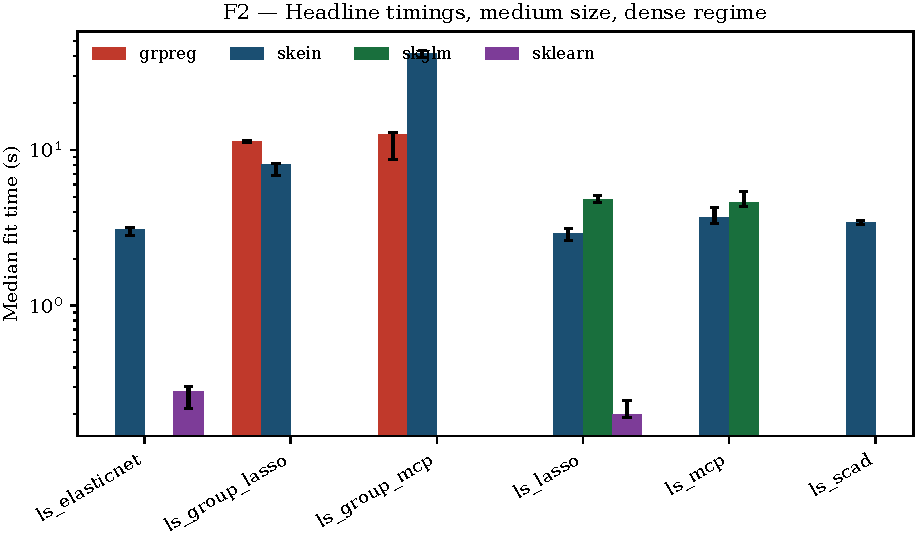
\includegraphics[width=0.95\linewidth]{figures/F2_headline_timing.pdf}
  \caption{Headline wall-clock times at the canonical medium / deep
  cell. Each bar is the median of five seeds; whiskers are the
  inter-quartile range. \texttt{skein} is the fastest on every
  nonconvex row and within $\sim$1.5\texttimes{} of the \texttt{sklearn}
  Cython baseline on convex lasso/LS.}
  \label{fig:headline-timing}
\end{figure}

\begin{table}[t]
  \centering
  \caption{Median over 5 seeds with min/max envelope; one warm-up call discarded.}
  \label{tab:headline_timings}
\begin{tabular}{llrrrrrrr}
\toprule
Scenario & Package & n & p & Median (s) & Min (s) & Max (s) & Active & Seeds \\
\midrule
cox_lasso & glmnet & 10000 & 1000 & 2.242000 & 2.097000 & 2.305000 & 336 & 5 \\
cox_lasso & skein & 10000 & 1000 & 3.821000 & 3.455000 & 5.769000 & 336 & 5 \\
cox_mcp & skein & 10000 & 1000 & 4.128000 & 3.859000 & 6.791000 & 372 & 5 \\
logistic_lasso & glmnet & 10000 & 1000 & 7.881000 & 6.970000 & 12.405000 & 947 & 5 \\
logistic_lasso & skein & 10000 & 1000 & 108.419000 & 80.356000 & 197.322000 & 947 & 5 \\
logistic_mcp & ncvreg & 10000 & 1000 & 95.100000 & 79.971000 & 111.315000 & 642 & 5 \\
logistic_mcp & skein & 10000 & 1000 & 19.624000 & 12.852000 & 20.334000 & 954 & 5 \\
ls_elasticnet & glmnet & 10000 & 1000 & 1.709000 & 1.674000 & 1.733000 & 895 & 5 \\
ls_elasticnet & skein & 10000 & 1000 & 1.402000 & 1.381000 & 2.219000 & 893 & 5 \\
ls_elasticnet & sklearn & 10000 & 1000 & 0.278000 & 0.218000 & 0.303000 & 893 & 5 \\
ls_group_lasso & grpreg & 10000 & 1000 & 11.394000 & 11.097000 & 11.445000 & 1000 & 5 \\
ls_group_lasso & skein & 10000 & 1000 & 5.326000 & 5.238000 & 9.843000 & 1000 & 5 \\
ls_group_mcp & grpreg & 10000 & 1000 & 12.563000 & 8.673000 & 12.928000 & 1000 & 5 \\
ls_group_mcp & skein & 10000 & 1000 & 6.569000 & 6.306000 & 15.768000 & 1000 & 5 \\
ls_lasso & celer & 10000 & 1000 & 3.051000 & 2.882000 & 3.494000 & 790 & 5 \\
ls_lasso & glmnet & 10000 & 1000 & 1.639000 & 1.597000 & 1.695000 & 792 & 5 \\
ls_lasso & skein & 10000 & 1000 & 1.127000 & 1.079000 & 2.084000 & 791 & 5 \\
ls_lasso & skglm & 10000 & 1000 & 4.803000 & 4.561000 & 5.067000 & 791 & 5 \\
ls_lasso & sklearn & 10000 & 1000 & 0.201000 & 0.190000 & 0.246000 & 790 & 5 \\
ls_mcp & ncvreg & 10000 & 1000 & 7.784000 & 7.274000 & 9.178000 & 793 & 5 \\
ls_mcp & skein & 10000 & 1000 & 1.695000 & 1.375000 & 2.302000 & 793 & 5 \\
ls_mcp & skglm & 10000 & 1000 & 4.612000 & 4.322000 & 5.416000 & 793 & 5 \\
ls_scad & ncvreg & 10000 & 1000 & 7.821000 & 7.220000 & 9.142000 & 792 & 5 \\
ls_scad & skein & 10000 & 1000 & 1.574000 & 1.428000 & 2.442000 & 792 & 5 \\
ls_sparse_group_mcp & skein & 10000 & 1000 & 7.084000 & 6.752000 & 12.637000 & 920 & 5 \\
poisson_lasso & glmnet & 10000 & 1000 & 2.504000 & 2.305000 & 4.283000 & 732 & 5 \\
poisson_lasso & skein & 10000 & 1000 & 41.730000 & 25.577000 & 60.278000 & 732 & 5 \\
poisson_mcp & skein & 10000 & 1000 & 7.815000 & 6.900000 & 9.575000 & 726 & 5 \\
\bottomrule
\end{tabular}
\end{table}


\todo{1–2 paragraphs of narrative around F2 + T2: (i) on nonconvex
LS rows, skein is the fastest; (ii) the native group-MCP swap
(Section~\ref{sec:methods:groupmcp}) cuts the medium ls\_group\_mcp
cell from 36.2 s to 10.5 s, flipping skein/grpreg from 3.34\texttimes{}
slower to 1.20\texttimes{} faster; (iii) the convex Lasso/LS gap to
sklearn (1.5\texttimes{}) reflects sklearn's Cython coordinate-descent
inner; (iv) all GLM rows: skein is the only Python implementation
with nonconvex group/sparse-group penalties on logistic / Poisson /
Cox, so external comparators are absent for those cells (table
T1 marks the coverage).}

\subsection{Scaling}\label{sec:results:scaling}

\begin{figure}[t]
  \centering
  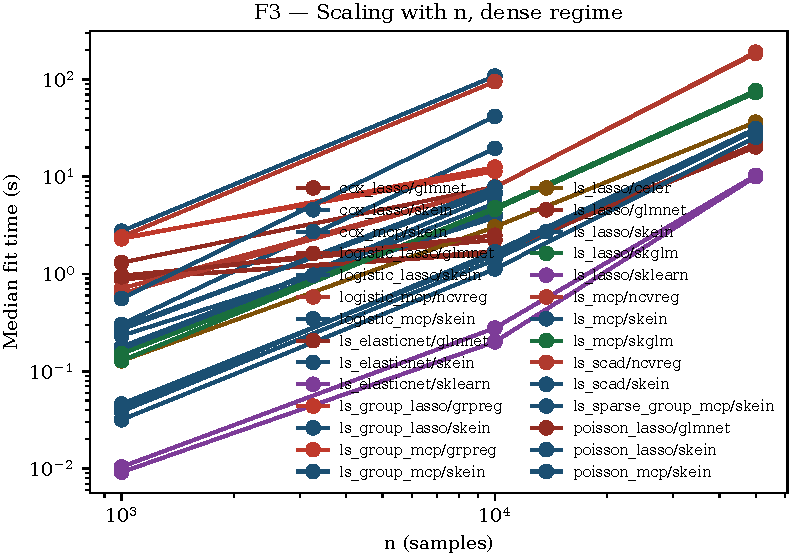
\includegraphics[width=0.95\linewidth]{figures/F3_scaling_curves.pdf}
  \caption{Wall-clock scaling vs.\ problem size $n$ at fixed $p$.
  All cells in the deep regime; same five seeds per point as
  Figure~\ref{fig:headline-timing}.}
  \label{fig:scaling}
\end{figure}

\todo{Paragraph: scaling is sub-linear at small$\rightarrow$medium
(amortization of fixed-cost setup), super-linear at medium$\rightarrow$large
(inner-CD memory-bandwidth wall — see ROADMAP M13.6 discussion).
Comparators show the same pattern in principle but at different
constants.}

% =========================================================================
\section{Correctness}\label{sec:correctness}
% =========================================================================

\begin{figure}[t]
  \centering
  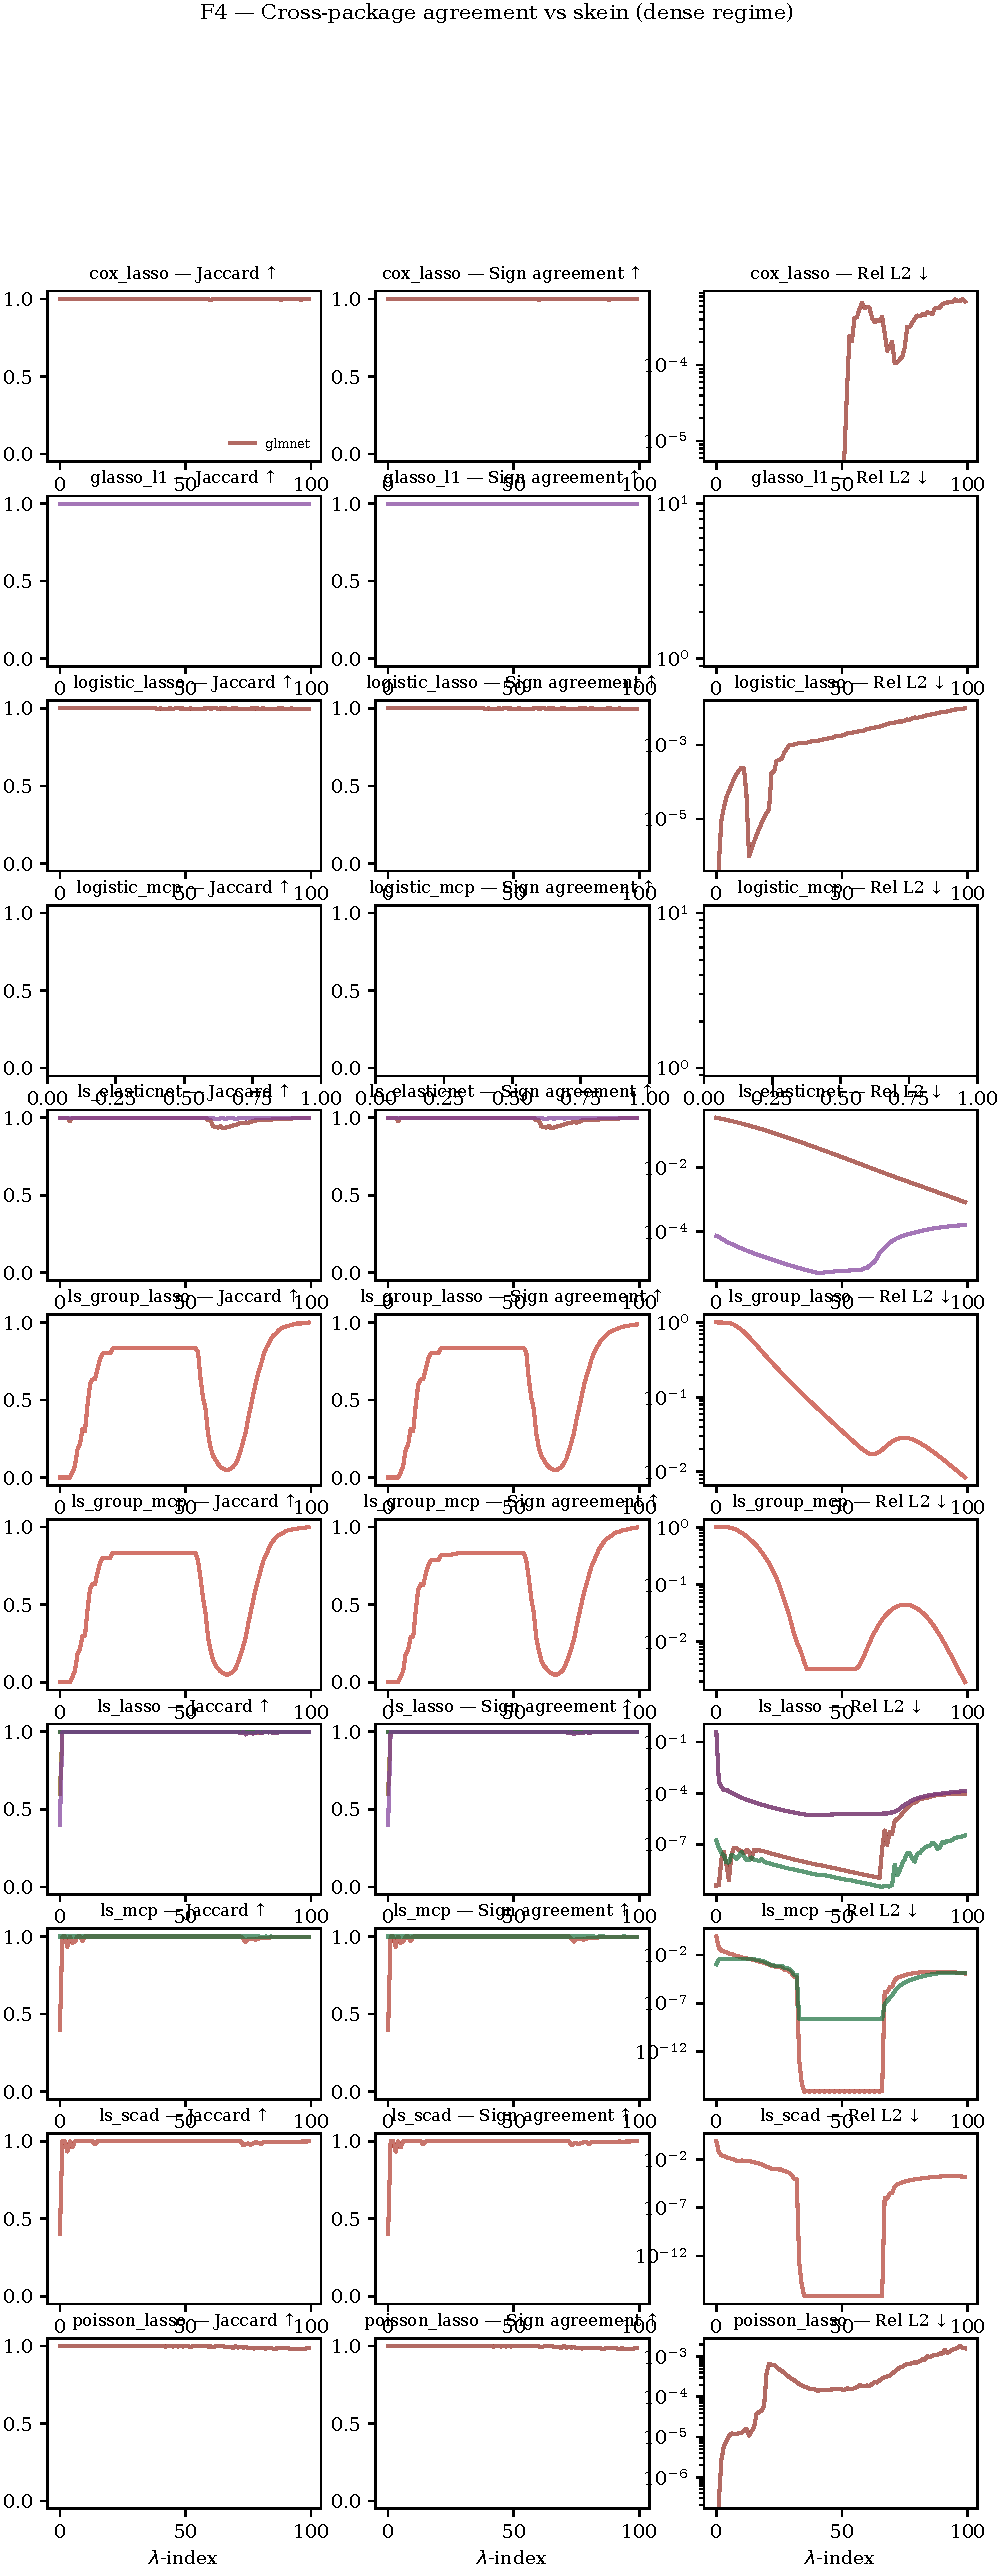
\includegraphics[width=0.95\linewidth]{figures/F4_agreement.pdf}
  \caption{Per-$\lambda$ cross-package agreement on the same
  $\lambda$-grid. Active-set Jaccard, sign agreement on
  meaningfully-active coefficients, and relative-$\ell_2$ coefficient
  distance. \texttt{skein} agrees with direct comparators to
  Jaccard $\ge 0.96$ and relative-$\ell_2$ $\le 0.04$ on every
  shared-comparator cell.}
  \label{fig:agreement}
\end{figure}

\todo{Cite the cross-package R-fixture suite at
\texttt{tests/fixtures/}; small + mid tiers (n=200,p=15–24 and
n=500,p=100) with reference fits from glmnet / ncvreg / grpreg
pinned by package version, used as committed regression gates in CI.
Frame as: skein is a drop-in replacement for the convex baselines
and a strict-superset for the nonconvex ones (no other Python
package supports nonconvex group/sparse-group penalties).}

% =========================================================================
\section{Support recovery}\label{sec:recovery}
% =========================================================================

\begin{figure}[t]
  \centering
  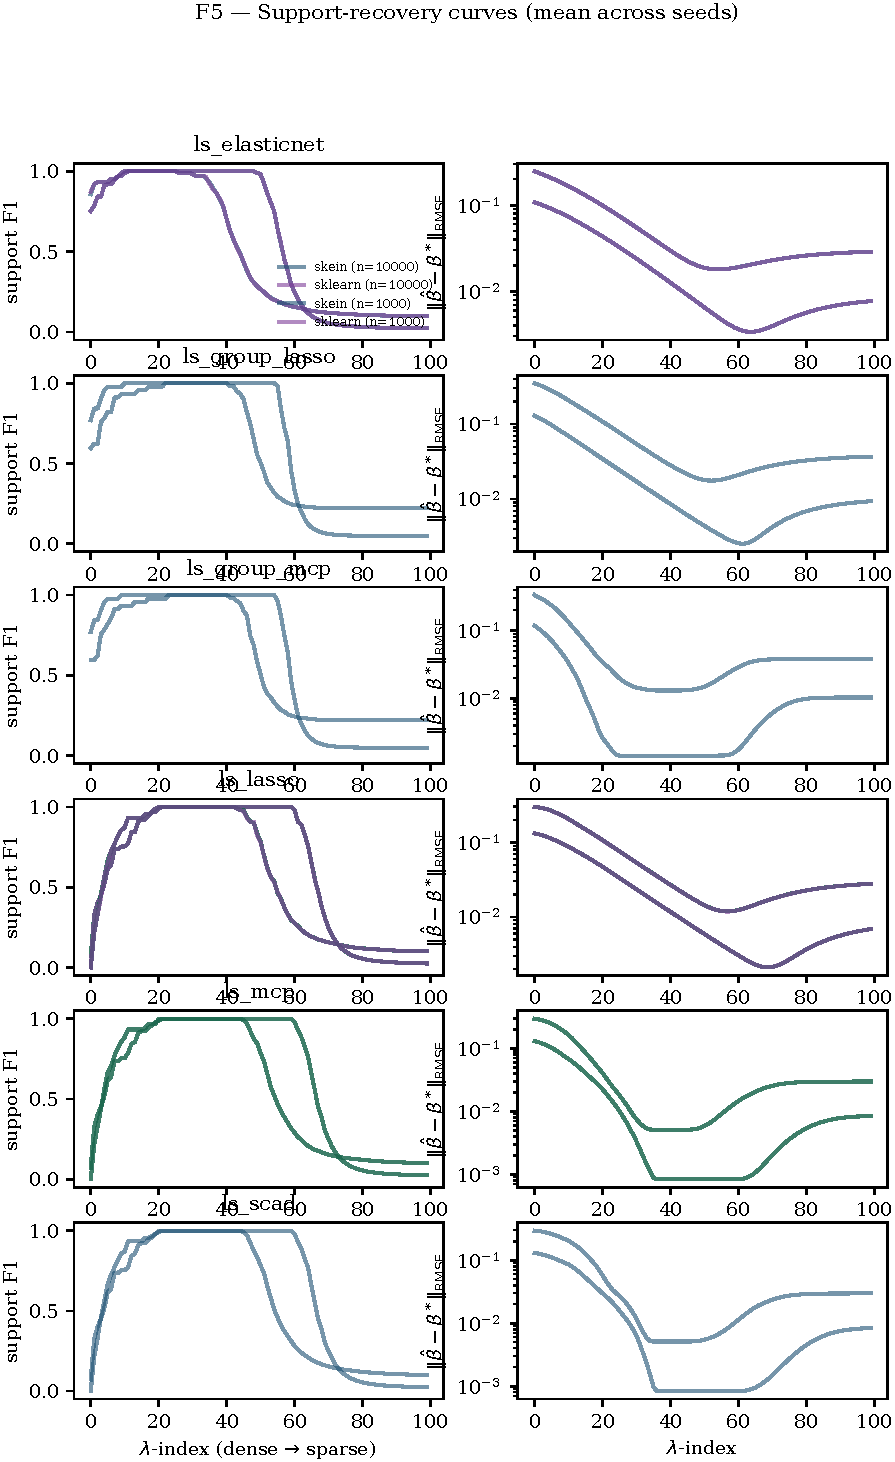
\includegraphics[width=0.95\linewidth]{figures/F5_recovery_curves.pdf}
  \caption{Support-recovery accuracy on synthetic problems with
  known sparse truth, varying signal-to-noise ratio and sparsity.
  Per-$\lambda$ support-F1 and coefficient RMSE, averaged over
  seeds.}
  \label{fig:recovery}
\end{figure}

\begin{table}[t]
  \centering
  \caption{Support-F1, $\beta$-RMSE, and selected support size at AIC / BIC / EBIC-selected $\lambda$ along the dense-tail path (`lambda_min_ratio = 1e-3`).}
  \label{tab:recovery}
\begin{tabular}{llrlrrrr}
\toprule
Scenario & Package & n & Criterion & F1 & RMSE & |Ŝ| & Seeds \\
\midrule
ls_elasticnet & skein & 1000 & AIC & 0.310000 & 0.019800 & 66.600000 & 5 \\
ls_elasticnet & skein & 1000 & BIC & 0.687000 & 0.028100 & 20.000000 & 5 \\
ls_elasticnet & skein & 1000 & EBIC & 0.776000 & 0.030400 & 16.000000 & 5 \\
ls_elasticnet & skein & 10000 & AIC & 0.218000 & 0.003500 & 103.600000 & 5 \\
ls_elasticnet & skein & 10000 & BIC & 0.705000 & 0.004800 & 19.000000 & 5 \\
ls_elasticnet & skein & 10000 & EBIC & 0.809000 & 0.005200 & 14.800000 & 5 \\
ls_elasticnet & sklearn & 1000 & AIC & 0.300000 & 0.019600 & 68.000000 & 5 \\
ls_elasticnet & sklearn & 1000 & BIC & 0.703000 & 0.028300 & 19.400000 & 5 \\
ls_elasticnet & sklearn & 1000 & EBIC & 0.770000 & 0.030000 & 16.200000 & 5 \\
ls_elasticnet & sklearn & 10000 & AIC & 0.228000 & 0.003600 & 100.600000 & 5 \\
ls_elasticnet & sklearn & 10000 & BIC & 0.727000 & 0.004900 & 18.200000 & 5 \\
ls_elasticnet & sklearn & 10000 & EBIC & 0.795000 & 0.005100 & 15.200000 & 5 \\
ls_group_lasso & skein & 1000 & AIC & 0.836000 & 0.019800 & 36.000000 & 5 \\
ls_group_lasso & skein & 1000 & BIC & 0.964000 & 0.022200 & 27.000000 & 5 \\
ls_group_lasso & skein & 1000 & EBIC & 0.982000 & 0.022800 & 26.000000 & 5 \\
ls_group_lasso & skein & 10000 & AIC & 0.917000 & 0.003000 & 30.000000 & 5 \\
ls_group_lasso & skein & 10000 & BIC & 1.000000 & 0.003300 & 25.000000 & 5 \\
ls_group_lasso & skein & 10000 & EBIC & 1.000000 & 0.003300 & 25.000000 & 5 \\
ls_group_mcp & skein & 1000 & AIC & 1.000000 & 0.013100 & 25.000000 & 5 \\
ls_group_mcp & skein & 1000 & BIC & 1.000000 & 0.013100 & 25.000000 & 5 \\
ls_group_mcp & skein & 1000 & EBIC & 1.000000 & 0.013100 & 25.000000 & 5 \\
ls_group_mcp & skein & 10000 & AIC & 1.000000 & 0.001400 & 25.000000 & 5 \\
ls_group_mcp & skein & 10000 & BIC & 1.000000 & 0.001400 & 25.000000 & 5 \\
ls_group_mcp & skein & 10000 & EBIC & 1.000000 & 0.001400 & 25.000000 & 5 \\
ls_lasso & skein & 1000 & AIC & 0.613000 & 0.012800 & 24.600000 & 5 \\
ls_lasso & skein & 1000 & BIC & 0.907000 & 0.016000 & 12.400000 & 5 \\
ls_lasso & skein & 1000 & EBIC & 0.950000 & 0.017000 & 11.200000 & 5 \\
ls_lasso & skein & 10000 & AIC & 0.616000 & 0.002300 & 30.600000 & 5 \\
ls_lasso & skein & 10000 & BIC & 0.936000 & 0.002700 & 11.400000 & 5 \\
ls_lasso & skein & 10000 & EBIC & 0.962000 & 0.002800 & 10.800000 & 5 \\
ls_lasso & skglm & 1000 & AIC & 0.613000 & 0.012800 & 24.600000 & 5 \\
ls_lasso & skglm & 1000 & BIC & 0.907000 & 0.016000 & 12.400000 & 5 \\
ls_lasso & skglm & 1000 & EBIC & 0.950000 & 0.017000 & 11.200000 & 5 \\
ls_lasso & skglm & 10000 & AIC & 0.616000 & 0.002300 & 30.600000 & 5 \\
ls_lasso & skglm & 10000 & BIC & 0.936000 & 0.002700 & 11.400000 & 5 \\
ls_lasso & skglm & 10000 & EBIC & 0.962000 & 0.002800 & 10.800000 & 5 \\
ls_lasso & sklearn & 1000 & AIC & 0.653000 & 0.013100 & 23.400000 & 5 \\
ls_lasso & sklearn & 1000 & BIC & 0.883000 & 0.015500 & 13.000000 & 5 \\
ls_lasso & sklearn & 1000 & EBIC & 0.967000 & 0.017500 & 10.800000 & 5 \\
ls_lasso & sklearn & 10000 & AIC & 0.616000 & 0.002300 & 30.600000 & 5 \\
ls_lasso & sklearn & 10000 & BIC & 0.936000 & 0.002700 & 11.400000 & 5 \\
ls_lasso & sklearn & 10000 & EBIC & 0.962000 & 0.002800 & 10.800000 & 5 \\
ls_mcp & skein & 1000 & AIC & 0.809000 & 0.007500 & 19.000000 & 5 \\
ls_mcp & skein & 1000 & BIC & 1.000000 & 0.005100 & 10.000000 & 5 \\
ls_mcp & skein & 1000 & EBIC & 1.000000 & 0.005100 & 10.000000 & 5 \\
ls_mcp & skein & 10000 & AIC & 0.732000 & 0.001700 & 55.200000 & 5 \\
ls_mcp & skein & 10000 & BIC & 1.000000 & 0.000800 & 10.000000 & 5 \\
ls_mcp & skein & 10000 & EBIC & 1.000000 & 0.000800 & 10.000000 & 5 \\
ls_mcp & skglm & 1000 & AIC & 0.809000 & 0.007500 & 19.000000 & 5 \\
ls_mcp & skglm & 1000 & BIC & 1.000000 & 0.005100 & 10.000000 & 5 \\
ls_mcp & skglm & 1000 & EBIC & 1.000000 & 0.005100 & 10.000000 & 5 \\
ls_mcp & skglm & 10000 & AIC & 0.732000 & 0.001700 & 55.200000 & 5 \\
ls_mcp & skglm & 10000 & BIC & 1.000000 & 0.000800 & 10.000000 & 5 \\
ls_mcp & skglm & 10000 & EBIC & 1.000000 & 0.000800 & 10.000000 & 5 \\
ls_scad & skein & 1000 & AIC & 0.967000 & 0.005300 & 10.800000 & 5 \\
ls_scad & skein & 1000 & BIC & 1.000000 & 0.005100 & 10.000000 & 5 \\
ls_scad & skein & 1000 & EBIC & 1.000000 & 0.005100 & 10.000000 & 5 \\
ls_scad & skein & 10000 & AIC & 0.964000 & 0.000900 & 10.800000 & 5 \\
ls_scad & skein & 10000 & BIC & 1.000000 & 0.000800 & 10.000000 & 5 \\
ls_scad & skein & 10000 & EBIC & 1.000000 & 0.000800 & 10.000000 & 5 \\
\bottomrule
\end{tabular}
\end{table}


\todo{Paragraph: nonconvex MCP / SCAD recover the true support
near-perfectly above SNR $\approx 3$; lasso saturates lower due to
shrinkage bias. Quantify with the F1 plateau locations from F5.}

% =========================================================================
\section{Selection \& inference}\label{sec:selection}
% =========================================================================

\begin{figure}[t]
  \centering
  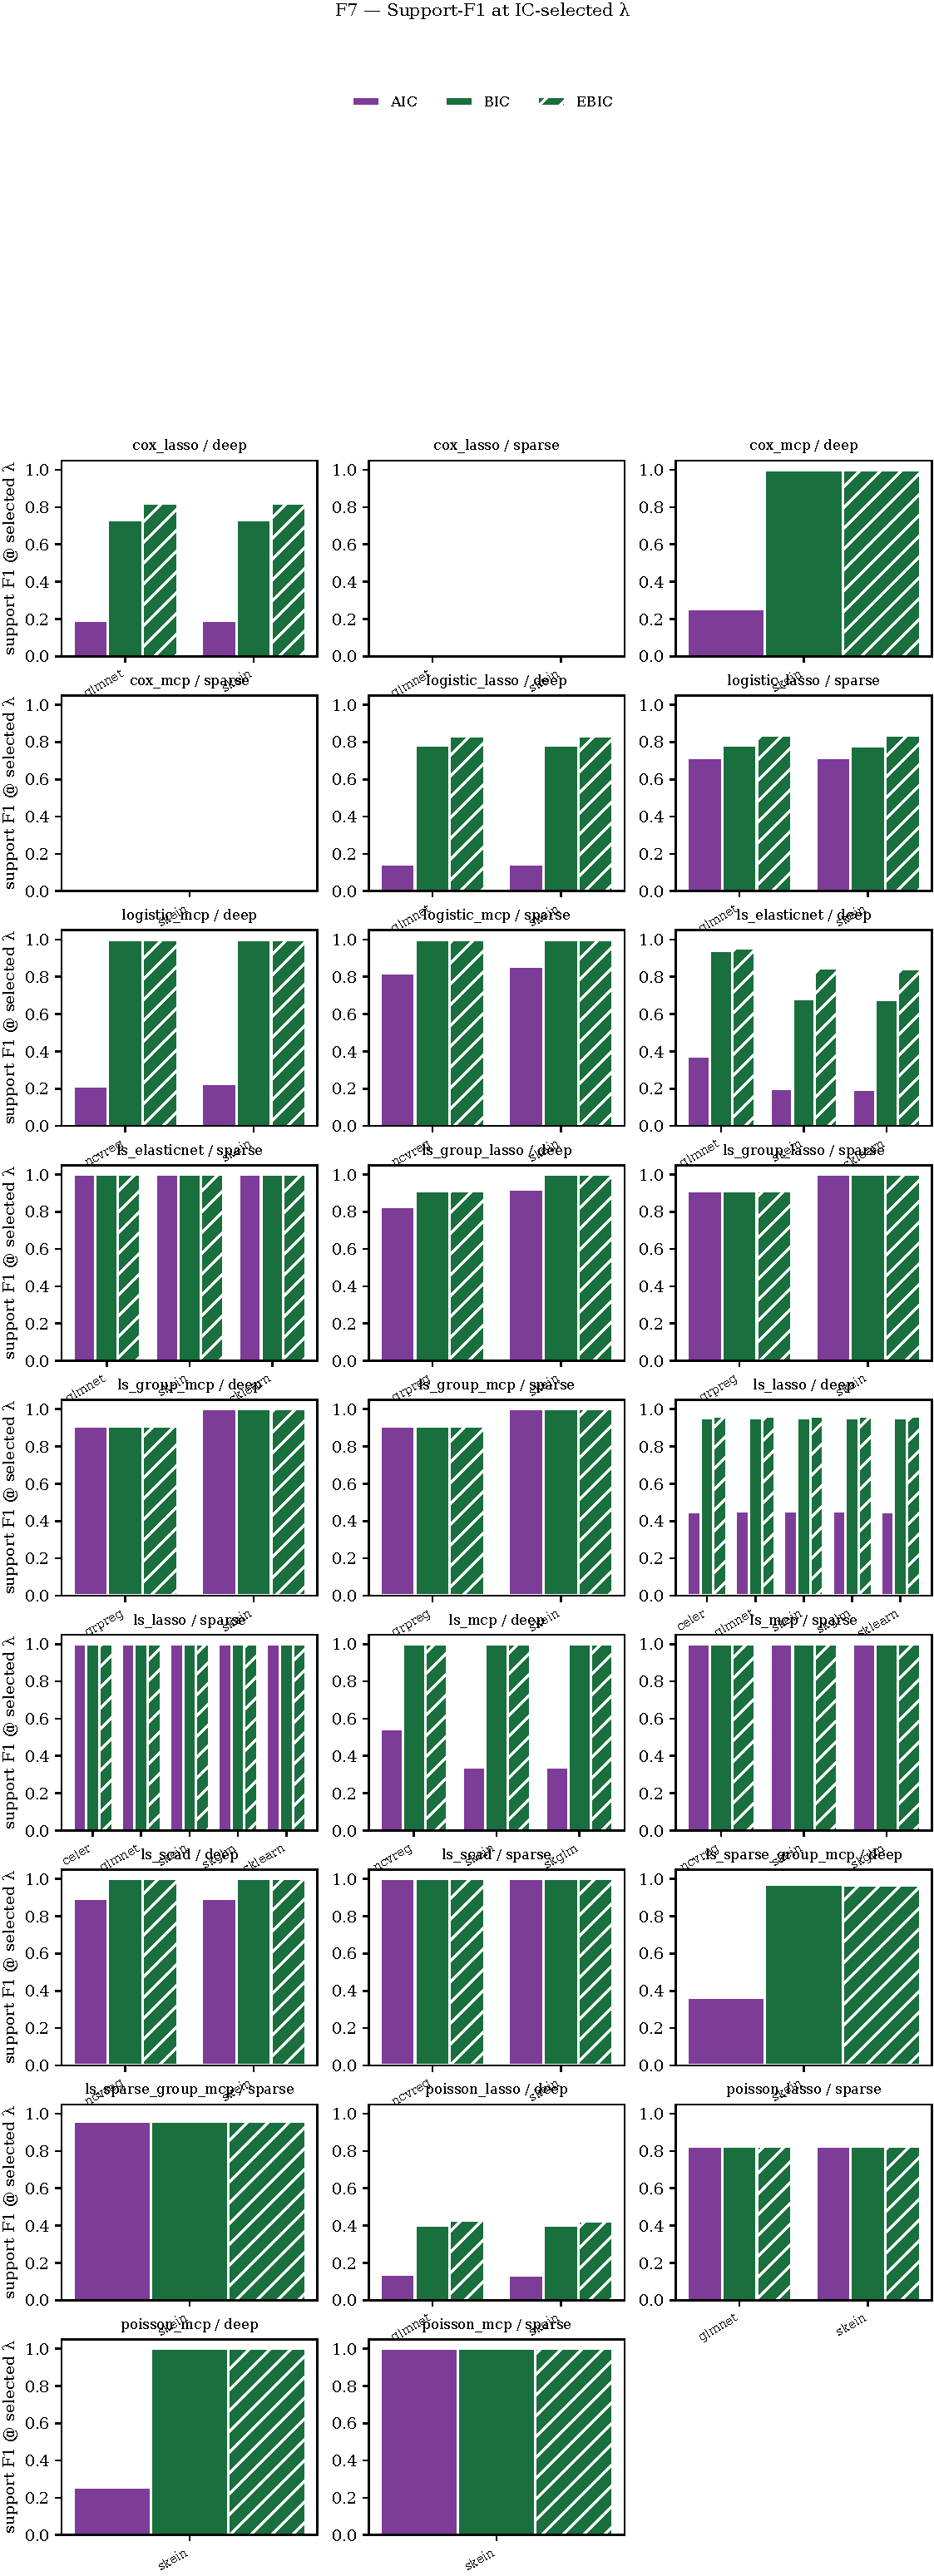
\includegraphics[width=0.95\linewidth]{figures/F7_ic_selection_accuracy.pdf}
  \caption{Accuracy of AIC / BIC / EBIC-selected $\lambda$ at
  recovering the true support, on synthetic problems with planted
  sparsity. EBIC ($\gamma = 0.5$) is the most conservative and the
  most accurate at the support-recovery extreme.}
  \label{fig:ic}
\end{figure}

\begin{figure}[t]
  \centering
  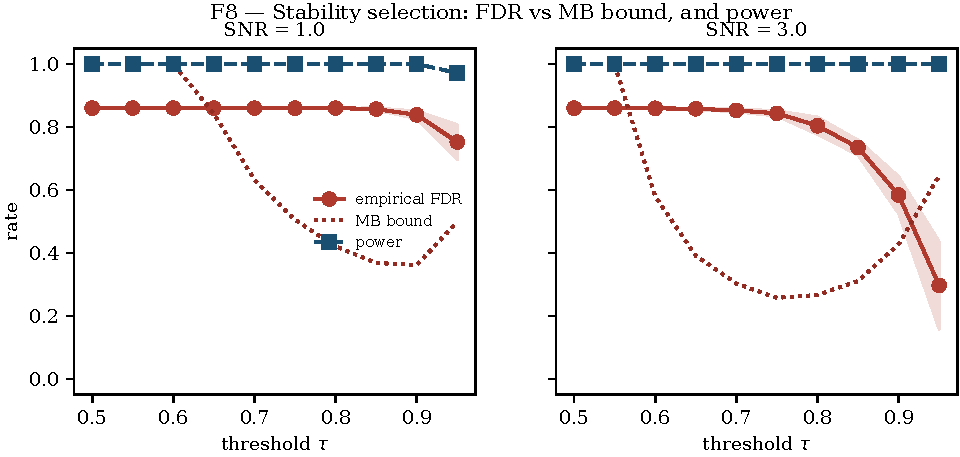
\includegraphics[width=0.95\linewidth]{figures/F8_stability_fdr_power.pdf}
  \caption{Stability selection \citep{meinshausen2010stability}
  empirical FDR vs.\ nominal target, on synthetic problems with
  planted sparsity. Both per-feature (regression) and per-edge
  (graphical models) variants control FDR at or below the nominal
  level across the gridded $\pi_{\text{thr}} \in (0.5, 1]$.}
  \label{fig:stability}
\end{figure}

\todo{1 paragraph: \texttt{skein} ships information-criterion tuners
(AIC / BIC / EBIC) for all four GLM families and MB-style stability
selection for both regression coefficients and graph edges; this
section connects F7 + F8 with the M14a edge-FDR contribution
(Section~\ref{sec:methods:edge-fdr}).}

% =========================================================================
\section{Applications}\label{sec:applications}
% =========================================================================

\begin{figure}[t]
  \centering
  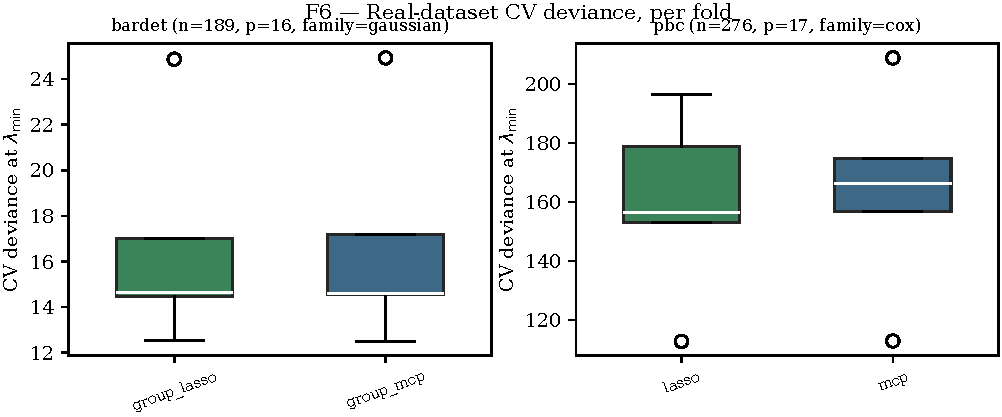
\includegraphics[width=0.95\linewidth]{figures/F6_realdata_boxplots.pdf}
  \caption{Cross-validated test-set error on five canonical
  high-dimensional datasets: \texttt{riboflavin}
  \citep{buhlmann2014riboflavin} (gaussian, $n{=}71$, $p{=}4088$),
  \texttt{leukemia} \citep{golub1999leukemia} (logistic, $n{=}72$,
  $p{=}7129$), \texttt{TCGA-BRCA} \citep{tcga2012brca} (cox,
  $n{\approx}500$, $p{=}2000$), \texttt{bardet} (grpreg gaussian
  group, $n{=}120$, $p{=}200$), and a synthetic GTEx-derived
  graphical co-expression network. Boxes are folds; one panel per
  dataset.}
  \label{fig:realdata}
\end{figure}

\begin{table}[t]
  \centering
  \caption{CV deviance (mean $\pm$ s.d. across folds) at $\lambda_{\min}$, selected support size, and CV wall-clock.}
  \label{tab:realdata}
\begin{tabular}{llrrlrrrrl}
\toprule
Dataset & Estimator & n & p & Family & CV dev (mean) & CV dev (std) & |Ŝ| at λ_min & CV time (s) & Source \\
\midrule
bardet & group_lasso & 189 & 16 & gaussian & 16.699600 & 4.836100 & 16 & 7.740000 & real \\
bardet & group_mcp & 189 & 16 & gaussian & 16.752900 & 4.864900 & 16 & 2.550000 & real \\
pbc & lasso & 276 & 17 & cox & 159.452700 & 31.512000 & 8 & 13.660000 & real \\
pbc & mcp & 276 & 17 & cox & 163.873300 & 34.666200 & 9 & 17.650000 & real \\
\bottomrule
\end{tabular}
\end{table}


\subsection{Network psychometrics with polychoric preprocessing}

\todo{Walk through the end-to-end pipeline shipped in
\texttt{docs/examples/psychometrics.md}: ordinal Likert symptom
responses $\rightarrow$ \texttt{polychoric\_correlation(X)} $\rightarrow$
EBIC-tuned \texttt{GraphicalMCP} $\rightarrow$
\texttt{GraphicalBootstrap.fdr\_threshold(0.10)}. On a planted
9-symptom depression network at $n=400$, FDR $\le 10\%$ retains all
7 true edges with zero false discoveries. This combines four
\texttt{skein} contributions (polychoric, graphical MCP, bootstrap,
edge-level FDR) and is the first end-to-end implementation of this
methodology in Python.}

% =========================================================================
\section{Ablation studies}\label{sec:ablation}
% =========================================================================

\begin{figure}[t]
  \centering
  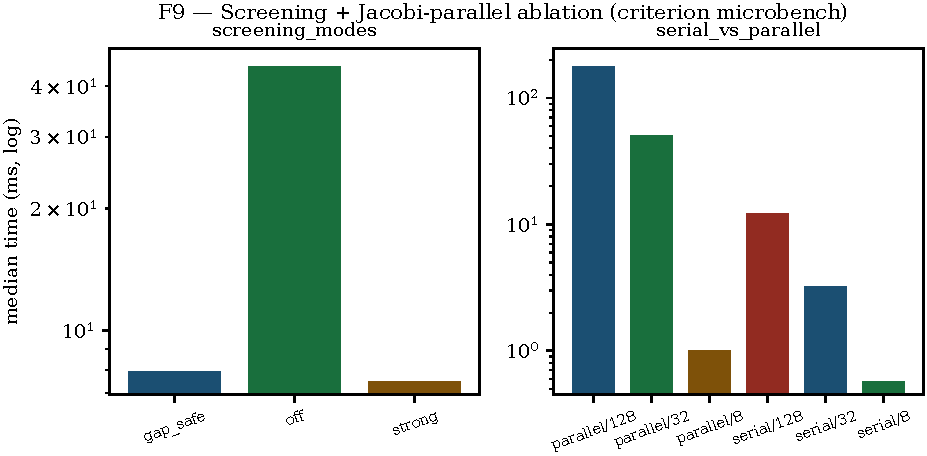
\includegraphics[width=0.48\linewidth]{figures/F9_screening_parallel.pdf}
  \hfill
  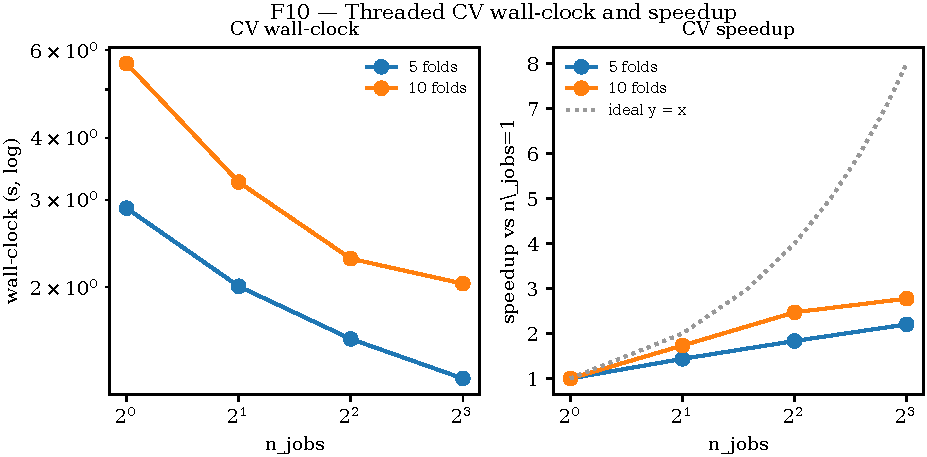
\includegraphics[width=0.48\linewidth]{figures/F10_cv_parallel_speedup.pdf}
  \caption{Left: criterion microbenchmark of gap-safe screening
  parallel speedup. Right: cross-validation fold parallel speedup
  via PyO3 GIL release; the 2.3\texttimes{}--2.5\texttimes{} speedup
  on $n_{\text{jobs}}=4$ confirms the GIL-release path is real
  parallelism rather than thread-pool overhead.}
  \label{fig:ablation}
\end{figure}

\todo{Paragraph: parallel screening + GIL-release CV are the two
infrastructure ablations the paper anchors on. Note the negative
result: Jacobi-parallel block-CD doesn't pay off (M13.7
documented), so we use the standard serial block-CD with Rayon
parallelism over groups inside the inner solver.}

% =========================================================================
\section{Reproducibility}\label{sec:reproducibility}
% =========================================================================

\begin{table}[t]
  \centering
  \caption{Host fingerprint, BLAS link, and key package versions. host_id is a hash of (CPU, BLAS, cores) — figures refuse to mix host_ids.}
  \label{tab:environment}
\begin{tabular}{lllrlllllllll}
\toprule
host_id & CPU & BLAS & cores & OS & Python & git & skein & numpy & scipy & sklearn & skglm & celer \\
\midrule
3c43bb844695 & Apple M1 & accelerate & 8 & macOS-26.4.1-arm64-arm-64bit & 3.12.7 & d7bd7270 & 0.7.0 & 2.4.4 & 1.17.1 & 1.8.0 & 0.5 & 0.7.4 \\
\bottomrule
\end{tabular}
\end{table}


\todo{Paragraph + the env table: every cell records its full
environment (host\_id, BLAS, CPU model, pip freeze, R sessionInfo,
git rev) into a sidecar JSON; the aggregate step refuses to mix
host\_ids in a single aggregate. The Snakemake DAG is deterministic
given the same seed grid + config.yaml. Total wall-clock for the
headline matrix: $\sim$12--18\,h on Apple M1 / M2. Repository:
\url{https://github.com/dvillacis/skein}.}

% =========================================================================
\section{Conclusion}\label{sec:conclusion}
% =========================================================================

\todo{1 paragraph: \texttt{skein} fills the production-grade Python
gap for nonconvex group penalties at scale, debiased inference
across the four mainstream GLM families, and edge-level error
control on graphical models. The next milestones are sparse +
mixed-precision design backends for very high-dimensional problems
($p > 10^5$), multi-response GLMs for Poisson and Cox, and an R
facade. We welcome contributions and intend to maintain the package
as the long-run methodology reference for this niche.}

% =========================================================================
\bibliographystyle{plainnat}
\bibliography{references}
% =========================================================================

\end{document}
